In the previous chapter, we have learned how an interpreted programming language can be implemented.
Another method of implementing a programming language is to create a compiler for this language.
However, the question of how such a compiler works exactly still remains.

\section{How a Compiler Translates the AST}

\begin{wrapfigure}{R}{0.52\textwidth}
	\centering
	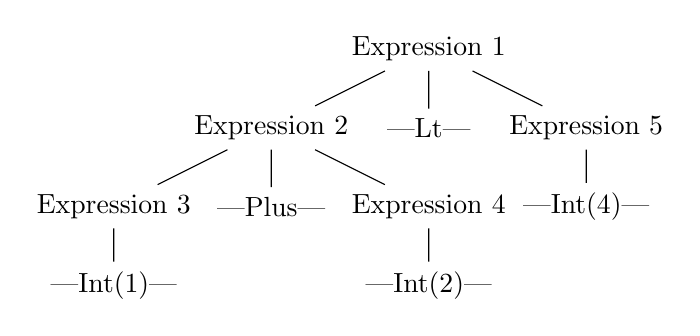
\begin{tikzpicture}[level distance=1cm, sibling distance=2cm]
		\node {Expression 1}
		child {node {Expression 2}
				child {node {Expression 3}
						child {node {\Verb|Int(1)|}}}
				child {node {\Verb|Plus|}}
				child {node {Expression 4}
						child {node {\Verb|Int(2)|}}}}
		child {node {\Verb|Lt|}}
		child {node {Expression 5}
				child {node {\Verb|Int(4)|}}};
	\end{tikzpicture}
	\caption{Abstract Syntax Tree for `\texttt{1+2 < 4}'}
	\label{fig:cmp_simple_tree}
\end{wrapfigure}

Often, a compiler traverses an AST created by the analyzer in order to generate some sort of output during the process.
For each AST node, the compiler usually calls a separate function or method which is specialized in translating this specific node type.
These individual functions often return some sort of value representing the translated node.
Otherwise, each individual function may also \emph{insert} generated instructions into an internal field of the compiler.
In these cases, each function often also returns metadata about the previously compiled node.
For instance, this data may include the register or memory location of a previously compiled expression, so that other AST nodes can refer to it later.
In transpires, meaning a compiler translating one high-level language into another one, each node-specific function often returns a tree node representing code in the output language.
For compilers which translate directly to instructions, each function often inserts its output into the instruction sequence directly.

Listing \ref{fig:cmp_simple_tree} displays a simplified syntax tree of the rush expression `\texttt{1+2 < 4}'.
In this example, compilation of the expression starts at the root node of the tree.
Here, most compilers will begin translation by first compiling the child nodes using some sort of \emph{post-order} traversal.
Post-order traversal is frequently used because the compilation of a node often depends on the output of its child nodes.
In this example, translation of the root comparison expression depends on the information returned by compiling its left- and right-hand sides.
Therefore, the compiler first considers the node `Expression 2' which represents the add-expression \texttt{1+2}.
Due to post-order traversal, the compiler first traverses the children of this node.
Here, the left child (`Expression 3') is traversed before the right child (`Expression 4') is traversed.
Since post-order traversal involves considering the current node at the end, the operand of `Expression 2' is considered at last.
Therefore, the instruction responsible for \texttt{1 + 2} is inserted after Expression node 3 and 4 have been traversed.
Since `Expression 2' is now completely traversed and its addition instruction has been inserted, the compiler now consideres the right-hand side of the comparison (`Expression 1').
Here, this node only consists of the constant integer value 4.
Now, all child nodes of `Expression\ have been traversed, thus the compiler now considers this node itself.
Here, the compiler notices that the expression should check if the left-hand side is less than the right-hand side.
Therefore, it inserts an instruction performing this comparison using the results of the left and right child as the operands.
In order to allow the add- and compare-expression to specify their operands,
each function actively involved in tree-traversal returns an entity describing the location of the runtime value of its previously compiled node.
For instance, such a describing entity can be the name of a register or the location of a variable in memory.
By returning information like this, a root node will have information about its children as soon as it is traversed.
Since this node then relies on the values of its child nodes, it is traversed after them, therefore creating the demand for post-order traversal.

\TSListing[raw=true, caption={Simple Pseudo-Instructions For a Fictional Architecture}, label={lst:cmp_simple_instructions}, float=H]{listings/simple_compiler_instructions.txt}

The instructions in Listing~\ref{lst:cmp_simple_instructions} display a sequence of instructions generated from the previously discussed tree for a fictional architecture.
It is apparent that the order of the instructions matches the order in which the tree was traversed.
The instructions responsible for the addition in the lines 1-3 are therefore inserted first.
Since the node `Expression 3' is traversed first, it also presents the first instruction.
Here, the value 1 is assigned to a register named `\texttt{r0}'.
Therefore, the `\texttt{add}' instruction in line 3 uses the \texttt{r0} and \texttt{r1} registers as its operands.
It is aware of its operand registers since the prior function calls for compiling the left- and right-hand side nodes returned their target registers.

